\section{Funkcija}

\begin{frame}
    \sectionpage
\end{frame}

\begin{frame}
    \tableofcontents[currentsection, hideothersubsections]
\end{frame}
        
\subsection{Funkcija}
        \begin{frame}
            \frametitle{Preslikava}

            \vskip-2em
            \begin{columns}
                \column{0.73\textwidth}
                    \only<2->{\begin{alertblock}{Preslikava}
                        \only<3->{Naj bosta $\mathcal{X}$ in $\mathcal{Y}$ neprazni množici. \\} 
                        \only<4->{\textbf{Preslikava} $f$ sestoji iz:}
                        \begin{itemize}
                            \item<5-> množice $\mathcal{X}$, ki ji pravimo \textbf{domena},
                            \item<6-> množice $\mathcal{Y}$, ki ji pravimo \textbf{kodomena} in 
                            \item<7-> \textbf{prirejanja}, ki vsakemu elementu $x$ domene priredi natanko en element $y$ kodomene.
                        \end{itemize}
                    \end{alertblock}}

                \column{0.24\textwidth}

                    \only<4->{\begin{alertblock}{}
                        $$\begin{aligned}
                            f&: \only<5->{\mathcal{X}}\only<6->{\to\mathcal{Y}} \\ \only<7->{f&: x\mapsto y}
                        \end{aligned}  $$
                    \end{alertblock}}
            
        \end{columns}

        \vskip-0.4em
        \only<8->{\begin{alertblock}{}
            Elemente $x$ kodomene $\mathcal{X}$ imenujemo \textbf{originali} preslikave.
             \only<9->{\\ Če elementu $x$ priredimo element $y$ iz kodomene, potem $y$ imenujemo \textbf{slika} elemeta $x$.}
        \end{alertblock}}

        \vskip-0.4em
        \only<10->{\begin{block}{}
            Preslikavo lahko podamo s predpisom, puščičnim diagramom, besednim opisom ...
        \end{block}}

        \end{frame}


        \begin{frame}
            \frametitle{Funkcija}

            \only<2->{\begin{alertblock}{Funkcija}
                \only<3->{Naj bosta $\mathcal{X}$ in $\mathcal{Y}$ neprazni številski množici. \\}
                \only<4->{\textbf{Funkcija} $f$ je preslikava med številskima množicama $\mathcal{X}$ in $\mathcal{Y}$:}
                \vskip-0.5em
                \only<5->{$$f: \mathcal{X}\to\mathcal{Y}.$$}
            \end{alertblock}}


            \only<6->{\begin{alertblock}{}
                Število $y$ je \textbf{funkcijska vrednost} števila $x$, če se število $x$ preslika v število $y$. 
                \vskip-0.5em
                \only<6->{$$ f(x)=y $$}
            \end{alertblock}}

            \only<7->{\begin{block}{}
                $x$ je neodvisna spremenjlivka, $f(x)$ je od $x$ odvisna spremenljivka.
            \end{block}}

        \end{frame}

        
        \begin{frame}
            
            \only<2->{\begin{block}{}
                V nekaterih primerih za opis funkcije uporabimo poseben izraz:
                \begin{itemize}
                    \item<3-> $f:\mathcal{X}\to\mathbb{R}; \mathcal{X}\subseteq\mathbb{R}$ -- realna funkcija realne spremenljivke;
                    \item<4-> $f:\mathcal{X}\to\mathbb{R}; \mathcal{X}\subseteq\mathbb{N}$ -- realna funkcija naravne spremenljivke;
                    \item<5-> $f:\mathcal{X}\to\mathbb{N}; \mathcal{X}\subseteq\mathbb{R}$ -- naravna funkcija realne spremenljivke;
                    \item<6-> $f:\mathcal{X}\to\mathbb{N}; \mathcal{X}\subseteq\mathbb{N}$ -- naravna funkcija naravne spremenljivke.
                \end{itemize}
            \end{block}}
        \end{frame}

        \begin{frame}
            \frametitle{Definicijsko območje in zaloga vrednosti}

            \only<2->{\begin{alertblock}{Definicijsko območje}
                \only<3->{\textbf{Definicijsko območje} preslikave ali funkcije $f:\mathcal{X}\to\mathcal{Y}$ je množica vseh originalov, ki jih v danem primeru opazujemo. 
                Oznaka: $D_f$.    }            
            \end{alertblock}}

            \vskip-0.5em
            \only<4->{\begin{block}{}
                Za definicijsko območje navadno vzamemo največjo možno množico, za katero je predpis funkcije veljaven/definiran.
            \end{block}}

            \only<5->{\begin{alertblock}{Zaloga vrednosti}
                \only<6->{\textbf{Zaloga vrednosti} preslikave ali funkcije $f:\mathcal{X}\to\mathcal{Y}$ je množica vseh slik oziroma funkcijskih vrednosti.
                Oznaka: $Z_f$.}
            \end{alertblock}}

            \vskip-0.5em
            \only<7->{\begin{block}{}
                Zaloga vrednosti $Z_f$ je podmnožica kodomene $\mathcal{Y}$: $Z_f\subseteq \mathcal{Y}$.
            \end{block}}

        \end{frame}



        %%%% naloge

        \begin{frame}

            \only<2->{\begin{exampleblock}{Naloga}
                Funkcijo $f: A\to B$ predstavite s tabelo. Izračunajte, kam posamezna funkcija preslika $x=1$.
                \begin{itemize}
                    \item $A=\left\{-2, -1, 0, 1, 2, 3\right\}$, $B=\left\{0, 1, 2, 3, 4, 5\right\}$, $f(x)=|x|+1$ \\~
                    \item $A=\left\{1, 2, 3, 4, 5\right\}$, $B=\mathbb{N}$, $f(x)=2x+1$ \\~
                    \item $A=B=\left\{\frac{1}{3}, \frac{1}{2}, 1, 2, 3\right\}$, $f(x)=\dfrac{1}{x}$ \\~
                \end{itemize} 
            \end{exampleblock}}
           
            \only<3->{\begin{exampleblock}{Naloga}
                Tabelirajte funkcijo $g(x)=2x+|x|$ od $-3$ do $3$ s korakom $1$. \\~
            \end{exampleblock}}


        \end{frame}


        \begin{frame}
            \only<2->{\begin{exampleblock}{Naloga}
                Zapišite definicijska območja funkcij.
                \vskip-0.5em
                \begin{columns}
                    \column{0.5\textwidth}
                    \begin{itemize}
                        \item $f(x)=\dfrac{-7}{x+1}$ \\~
                        \item $g(x)=\dfrac{1}{(x+2)(x+6)}$ \\~
                        \item $h(x)=\dfrac{3x^2+1}{5}$ \\~
                        \item $i(x)=\sqrt{x-2}$ \\~
                    \end{itemize}

                    \column{0.47\textwidth}
                    \begin{itemize}
                        \item $j(x)=x^3-\frac{2}{3}$ \\~
                        \item $k(x)=\sqrt{x^2+7}$ \\~
                        \item $l(x)=\dfrac{3}{x}$ \\~
                        \item $m(x)=\dfrac{x^2+1}{x^2-5x-6}$ \\~
                    \end{itemize}
                \end{columns}

            \end{exampleblock}}
        \end{frame}

        %%%%%%%%%%%%%%%%%%%%%%%%%%%%%%%%%%%%%%%%%%%%%%%%


        \begin{frame}
            \frametitle{Ničla in začetna vrednost funkcije}

            \only<2->{\begin{alertblock}{Ničla funkcije}
                \only<3->{\textbf{Ničla} funkcije $f:\mathcal{X}\to\mathcal{Y}$ je tista vrednost $x_0\in\mathcal{X}$ neodvisne spremenljivke, 
                pri kateri je vrednost funkcije $f$ enaka $0$: $f(x_0)=0$.}
            \end{alertblock}}

            \vskip-0.5em
            \only<4->{\begin{block}{}
                Ničle funkcije $f$ poiščemo tako, da rešimo enačbo $f(x)=0$. \\
                \only<5->{Ničle so le tiste izmed vrednosti, ki ležijo v definicijskem območju $D_f$ funkcije $f$.}
            \end{block}}

            \only<6->{\begin{alertblock}{Začetna vrednost}
                \only<7->{\textbf{Začetna vrednost} funkcije $f:\mathcal{X}\to\mathcal{Y}$ je funkcijska vrednost pri $x=0$, to je $f(0)$.}
            \end{alertblock}}

            \vskip-0.5em
            \only<8->{\begin{block}{}
                Začetna vrednost obstaja le, če je $0$ v definicijskem območju funkcije $f$: $0\in D_f$.
            \end{block}}
        \end{frame}



        %%%% naloge

        \begin{frame}
            \only<2->{\begin{exampleblock}{Naloga}
                Izračunajte ničle funkcij.
                \vskip-0.5em
                \begin{columns}
                    \column{0.5\textwidth}
                    \begin{itemize}
                        \item $f(x)=\frac{4}{5}-6x$ \\~
                        \item $g(x)=x^2-7x+12$ \\~
                        \item $h(x)=\dfrac{3x+6}{5}$ \\~
                        \item $i(x)=x^2-9$ \\~
                    \end{itemize}

                    \column{0.47\textwidth}
                    \begin{itemize}
                        \item $j(x)=x^2+1$ \\~
                        \item $k(x)=x^2-3x^2-4x+12$ \\~
                        \item $l(x)=\sqrt{x+7}$ \\~
                        \item $m(x)=\dfrac{3}{x}$ \\~
                    \end{itemize}
                \end{columns}

            \end{exampleblock}}
        \end{frame}


        \begin{frame}
            \only<2->{\begin{exampleblock}{Naloga}
                Izračunajte začetne vrednosti funkcij.
                \vskip-0.5em
                \begin{columns}
                    \column{0.5\textwidth}
                    \begin{itemize}
                        \item $f(x)=\frac{4}{5}-6x$ \\~
                        \item $g(x)=x^2-7x+12$ \\~
                        \item $h(x)=\dfrac{3x+6}{5}$ \\~
                        \item $i(x)=x^2-9$ \\~
                    \end{itemize}

                    \column{0.47\textwidth}
                    \begin{itemize}
                        \item $j(x)=x^2-3x^2-4x+12$ \\~
                        \item $k(x)=\sqrt{x+7}$ \\~
                        \item $l(x)=\dfrac{3}{x}$ \\~
                        \item $m(x)=\dfrac{x^3-2x^2-4}{x^4+2x^3+3}$ \\~
                    \end{itemize}
                \end{columns}

            \end{exampleblock}}
        \end{frame}


        %%%%%%%%%%%%%%%%%%%%%%%%%%%%%%%


        \begin{frame}
            \frametitle{Graf funkcije}

            \only<2->{\begin{alertblock}{Graf funkcije}
                \only<3->{\textbf{Graf} $\Gamma_f$ funkcije $f:\mathcal{X}\to\mathcal{Y}$ je množica urejenih parov $(x,y)\in\mathcal{X}\times\mathcal{Y}$, 
                kjer element $x$ preteče celotno definicijsko območje $D_f$ funkcije, element $y$ pa je slika pripadajočega $x$, torej $y=f(x)$.}
                \only<4->{$$ \Gamma_f=\left\{(x,y)\in\mathcal{X}\times\mathcal{Y}; x\in D_f \land y=f(x)\right\} $$}
            \end{alertblock}}

            \only<5->{\begin{block}{}
                Urejene pare iz množice $\Gamma_f$ lahko upodobimo v koordinatnem sistemu. \\
                \only<6->{Vsakemu elementu $(x,f(x))$ iz zgornje množice pripada natanko ena točka v koordinatnem sistemu, 
                katere abscisa je enaka $x$, ordinata pa je njegova slika $f(x)$.}
            \end{block}}

            \only<7->{\begin{block}{}
                V ničli graf funkcije seka abscisno os, v začetni vrednosti pa ordinatno os.
            \end{block}}
        \end{frame}


        %%%%%%%%%%%%%%%%%%%

        \begin{frame}
            \frametitle{Naraščanje in padanje}

            \only<2->{\begin{alertblock}{Naraščajoča funkcija}
                \only<3->{Funkcija $f$ je na intervalu $(a,b)$ \textbf{naraščajoča}, če za poljubna $x_1,x_2\in(a,b)$, kjer je $x_1<x_2$, velja $f(x_1)\leq f(x_2)$.}
                
                \only<4->{Funkcija $f$ je na intervalu $(a,b)$ \textbf{strogo naraščajoča}, če za poljubna $x_1,x_2\in(a,b)$, kjer je $x_1<x_2$, velja $f(x_1)<f(x_2)$.}
            \end{alertblock}}

            \only<5->{\begin{alertblock}{Padajoča funkcija}
                \only<6->{Funkcija $f$ je na intervalu $(a,b)$ \textbf{padajoča}, če za poljubna $x_1,x_2\in(a,b)$, kjer je $x_1<x_2$, velja $f(x_1)\geq f(x_2)$.}
                
                \only<7->{Funkcija $f$ je na intervalu $(a,b)$ \textbf{strogo padajoča}, če za poljubna $x_1,x_2\in(a,b)$, kjer je $x_1<x_2$, velja $f(x_1)>f(x_2)$.}
            \end{alertblock}}

        \end{frame}


        %%%%%%%%%%%%

        \begin{frame}
            \frametitle{Injektivnost in surjektivnost}

            \vskip-1em
            \only<2->{\begin{alertblock}{Surjektivnost}
                \only<3->{Funkcija $f:\mathcal{X}\to\mathcal{Y}$ je \textbf{surjektivna}, če je zaloga vrednosti $Z_f$ funkcije enaka njeni kodomeni $\mathcal{Y}$ -- vsak element kodomene $\mathcal{Y}$ je slika vsaj enega elementa iz domene $\mathcal{X}$.}
                \vskip-1em
                \only<4->{$$\forall y\in\mathcal{Y}. \exists x\in\mathcal{X}\ni:f(x)=y$$}
            \end{alertblock}}

            \vskip-0.3em
            \only<5->{\begin{alertblock}{Injektivnost}
                \only<6->{Funkcija $f:\mathcal{X}\to\mathcal{Y}$ je \textbf{injektivna}, če se dva poljubna različna originala iz domene $\mathcal{X}$ preslikata v različni sliki v kodomeni $\mathcal{Y}$ -- vsak element kodomene $\mathcal{Y}$ je slika kvečjemu enega elementa iz domene $\mathcal{X}$.}
                \vskip-1em
                \only<7->{$$\forall x,y\in\mathcal{X}: f(x)=f(y)\Rightarrow x=y$$}
            \end{alertblock}}

            \vskip-0.5em
            \only<8->{\begin{alertblock}{}
                Funkcija $f:\mathcal{X}\to\mathcal{Y}$ je \textbf{bijektivna}, če je injektivna in surjektivna hkrati -- vsak element iz kodomene $\mathcal{Y}$ je slika natanko enega elementa domene $\mathcal{X}$.
            \end{alertblock}}
        \end{frame}


            %%%% naloge

            \begin{frame}
                \only<2->{\begin{exampleblock}{Naloga}
                    Zapišite in narišite grafe funkcij ter zapišite začetne vrednosti in ničle funkcije.
                    Določite, kje je funkcija naraščajoča oziroma padajoča, ter preverite surjektivnost in injektivnost.
                        \begin{itemize}
                            \item $f(x)=x \quad \quad D_f=\mathbb{R}$ \\~
                            \item $g(x)=-2x+1 \quad \quad D_g=\mathbb{R}$ \\~
                            \item $h(x)=x^2-1 \quad \quad D_h=\mathbb{R}$ \\~
                            \item $i(x)=\dfrac{1}{x^2} \quad \quad D_i=\left\{-2, -1, -\frac{1}{2}, \frac{1}{2}, 1, 2\right\}$ \\~
                            \item $j(x)=\dfrac{x+2}{x-3} \quad \quad D_j=\left\{-2, -1, 0, 1, 2\right\}$ \\~
                        \end{itemize}
                \end{exampleblock}}
            \end{frame}
        

        %%%%%%%%%%%%%%%%%%%%%%%%%%%%




        \subsection{Linearna funkcija}

        \begin{frame}
            \frametitle{Predpis linearne funkcije}
        \end{frame}


        %%% naloge

        \begin{frame}
            \only<2->{\begin{exampleblock}{Naloga}
                Ugotovite, ali je dana funkcija linearna. Linearnim funkcijam določite smerni koeficient in začetno vrednost.
                \vskip-0.5em
                \begin{columns}
                    \column{0.5\textwidth}
                    \begin{itemize}
                        \item $f(x)=\dfrac{1}{7x}-\dfrac{3}{4}$ \\~
                        \item $g(x)=\dfrac{2}{3}-\pi x$ \\~
                        \item $h(x)=\dfrac{8+6x}{24}$ \\~
                        \item $i(x)=0.\overline{3}x+1$ \\~
                    \end{itemize}

                    \column{0.47\textwidth}
                    \begin{itemize}
                        \item $j(x)=\dfrac{x^2-3}{5}$ \\~
                        \item $k(x)=-\sqrt{2}x+\dfrac{2}{3}$ \\~
                        \item $l(x)=2$ \\~
                    \end{itemize}
                \end{columns}

            \end{exampleblock}}
        \end{frame}



        \begin{frame}
            \only<2->{\begin{exampleblock}{Naloga}
                Zapišite predpis linearne funkcije $f$, ki ima začetno vrednost $5$ in diferenčni količnik $-3$. \\~
            \end{exampleblock}}

            \only<3->{\begin{exampleblock}{Naloga}
                Dana je linearna funkcija $p(x)=3x-4$. Izračunajte $p(-2)$, $p(0)$; $p(5)$ in $p(\sqrt{2})$. \\~
            \end{exampleblock}}

            \only<4->{\begin{exampleblock}{Naloga}
                Zapišite predpis linearne funkcije, za katero je $u(-2)=10$ in $u(0)=2$. \\~
            \end{exampleblock}}

        \end{frame}


        \begin{frame}
            \only<2->{\begin{exampleblock}{Naloga}
                Ali je funkcija naraščajoča ali padajoča?
                \vskip-0.5em
                \begin{columns}
                    \column{0.5\textwidth}
                    \begin{itemize}
                        \item $f(x)=3x+5$ \\~
                        \item $g(x)=-2x+7$ \\~
                        \item $h(x)=10-\frac{1}{2}x$ \\~
                        \item $i(x)=\dfrac{x-1}{2}$ \\~
                    \end{itemize}

                    \column{0.47\textwidth}
                    \begin{itemize}
                        \item $j(x)=\dfrac{5-2x}{3}$ \\~
                        \item $k(x)=\dfrac{-\sqrt{3}x+1}{3}$ \\~
                        \item $l(x)=-\dfrac{2-4x}{17}$ \\~
                    \end{itemize}
                \end{columns}

            \end{exampleblock}}
        \end{frame}


        \begin{frame}
            \only<2->{\begin{exampleblock}{Naloga}
                Izračunajte ničlo linearne funkcije.
                \vskip-1.5em
                \begin{columns}
                    \column{0.5\textwidth}
                    \begin{itemize}
                        \item $f(x)=6x+12$ \\~
                        \item $g(x)=5x+2$ \\~
                        \item $h(x)=3x-12$ \\~
                        \item $i(x)=-4x+8$ \\~
                        \item $j(x)=-3x+2$ \\~
                        \item $k(x)=-x-7$ \\~
                    \end{itemize}

                    \column{0.47\textwidth}
                    \begin{itemize}
                        \item $l(x)=\frac{3}{4}x-\frac{1}{4}$ \\~
                        \item $m(x)=-\dfrac{2x+3}{6}$ \\~
                        \item $n(x)=\dfrac{1-4x}{2}$ \\~
                        \item $o(x)=\dfrac{\pi x+4}{3}$ \\~
                        \item $p(x)=\sqrt{2}x+1$ \\~
                        \item $r(x)=4$ 
                    \end{itemize}
                \end{columns}

            \end{exampleblock}}
        \end{frame}


        \begin{frame}
            \only<2->{\begin{exampleblock}{Naloga}
                Dana je linearna funkcija $f$. Zapišite predpis funkcije $g$ v obliki $g(x)=kx+n$.
                    \begin{itemize}
                        \item $f(x)=2x-6, ~ g(x)=3f(x)$ \\~
                        \item $f(x)=5x-3; ~ g(x)=f(x+1)$ \\~
                        \item $f(x)=\dfrac{2x-5}{3}; ~ g(x)=f(1-x)$ \\~
                        \item $f(x)=\dfrac{10-4x}{7}; ~ g(x)=f(3x)$ \\~
                    \end{itemize}
            \end{exampleblock}}
        \end{frame}


        \begin{frame}
            \only<2->{\begin{exampleblock}{Naloga}
                Dana je družina linearnih funkcij $f(x)=(2m-1)x+(3-m); ~m\in\mathbb{R}$.
                    \begin{itemize}
                        \item Za katero vrednost parametra $m$ ima funkcija diferenčni količnik enak $-5$? 
                        \item Za katero vrednost parametra $m$ je funkcija padajoča?
                        \item Za katero vrednost parametra $m$ je funkcija konstantna? 
                        \item Za katero vrednost parametra $m$ je funkcija naraščajoča? 
                        \item Za katero vrednost parametra $m$ je začetna vrednost enaka $2$? 
                        \item Za katero vrednost parametra $m$ ima funkcija ničlo $x=-4$? 
                    \end{itemize}
            \end{exampleblock}}
        \end{frame}


        \begin{frame}
            \only<2->{\begin{exampleblock}{Naloga}
                Taksist meri razdaljo, ki jo je prevozil. Vsak kilometer stane $2.5~€$, startnina pa $7~€$.
                Zapišite funkcijo, po kateri taksist izračuna znesek za plačilo, ko prebere število prevoženih kilometrov $x$. 
                Izračunajte, koliko bi pačali, če bi se peljali $12~km$. \\~\\~
            \end{exampleblock}}

            \only<3->{\begin{exampleblock}{Naloga}
                V bezenu je $12~l$ vode. V bazen po cevi vsako minuto pritečejo še $4~l$ vode.
                Zapišite funkcijo, s katero bomo lahko izračunali, koliko je vode v bazenu po pretečenih $x$ minutah.
                Izračunajte, koliko vode je v bazenu po $9$ minutah. \\~\\~
            \end{exampleblock}}


        \end{frame}






    \subsection{Graf linearne funkcije}

        \begin{frame}
            \frametitle{Graf linearne funkcije}
        \end{frame}


        \begin{frame}
            \only<2->{\begin{exampleblock}{Naloga}
                Katere od točk $A(1,1)$, $B(4,0)$, $C(7,-2)$, $D(-4,\frac{5}{2})$, $E(0,\frac{3}{2})$, $F(2,2)$ in $G(3,0)$ ležijo na grafu funkcije $f(x)=-\frac{1}{2}x+\frac{3}{2}$? \\~\\~
            \end{exampleblock}}

            \only<3->{\begin{exampleblock}{Naloga}
                Dana je funkcija $g(x)=3x-2$. Za koliko se spremeni vrednost funkcije $g$, če se vrednost $x$
                \begin{itemize}
                    \item poveča za $1$?
                    \item poveča za $2$?
                    \item zmanjša za $5$?
                    \item zmanjša za $-10$?
                \end{itemize} 
            \end{exampleblock}}

        \end{frame}


        \begin{frame}
            \only<2->{\begin{exampleblock}{Naloga}
                Narišite graf linearne funkcije. Zapišite začetno vrednost in izračunajte ničlo funkcije.
                Določite, kje je funkcija pozitivna oziroma negativna, ter ali je naraščajoča ali padajoča?
                \vskip-1em
                \begin{columns}
                    \column{0.5\textwidth}
                    \begin{itemize}
                        \item $f(x)=-x+\frac{1}{2}$ \\~
                        \item $g(x)=2x+2$ \\~
                        \item $h(x)=3-2x$ \\~
                        \item $i(x)=-x$ \\~
                    \end{itemize}

                    \column{0.47\textwidth}
                    \begin{itemize}
                        \item $j(x)=-3$ \\~
                        \item $k(x)=\dfrac{6x-1}{3}$ \\~
                        \item $l(x)=-\dfrac{2-3x}{4}$ \\~
                        \item $m(x)=3-\frac{3}{5}x$ \\~
                    \end{itemize}
                \end{columns}

            \end{exampleblock}}
        \end{frame}


        \begin{frame}
            \only<2->{\begin{exampleblock}{Naloga}
                V isti koordinatni sistem narišite grafe funkcij $f(x)=2x-2$, $g(x)=2x+1$, $h(x)=2x+2$ in $i(x)=2x$.
                Kaj opazite? \\~\\~
            \end{exampleblock}}

            \only<3->{\begin{exampleblock}{Naloga}
                V isti koordinatni sistem narišite grafe funkcij $f(x)=2x-2$, $g(x)=3x-2$, $h(x)=x-2$ in $i(x)=\frac{1}{2}x-2$.
                Kaj opazite? \\~\\~
            \end{exampleblock}}

        \end{frame}


        \begin{frame}
            \only<2->{\begin{exampleblock}{Naloga}
                Zapišite predpis linearne funkcije, ki jo prikzauje graf.

                \begin{columns}
                    \column{0.32\textwidth}
                    \vskip-1.5em
                    \begin{figure}[H]
                        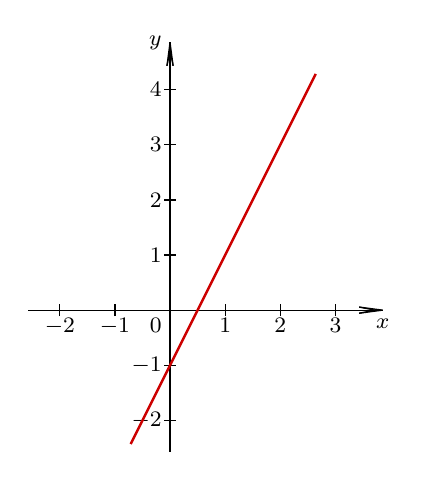
\begin{tikzpicture}
                            % \clip (0,0) rectangle (14.000000,10.000000);
                            {\footnotesize
                            
                            % Drawing 2D Cartesian system
                            \draw (3.000000,3.000000) node [anchor=north east] { $0$ };%
                            \draw [line width=0.016cm] (3.000000,2.925000) -- (3.000000,3.075000);%
                            \draw (3.700000,3.000000) node [anchor=north] { $1$ };%
                            \draw [line width=0.016cm] (3.700000,2.925000) -- (3.700000,3.075000);%
                            \draw (4.400000,3.000000) node [anchor=north] { $2$ };%
                            \draw [line width=0.016cm] (4.400000,2.925000) -- (4.400000,3.075000);%
                            \draw (5.100000,3.000000) node [anchor=north] { $3$ };%
                            \draw [line width=0.016cm] (5.100000,2.925000) -- (5.100000,3.075000);%
                            \draw (2.300000,3.000000) node [anchor=north] { $-1$ };%
                            \draw [line width=0.016cm] (2.300000,2.925000) -- (2.300000,3.075000);%
                            \draw (1.600000,3.000000) node [anchor=north] { $-2$ };%
                            \draw [line width=0.016cm] (1.600000,2.925000) -- (1.600000,3.075000);%
                            \draw (3.000000,3.700000) node [anchor=east] { $1$ };%
                            \draw [line width=0.016cm] (2.925000,3.700000) -- (3.075000,3.700000);%
                            \draw (3.000000,4.400000) node [anchor=east] { $2$ };%
                            \draw [line width=0.016cm] (2.925000,4.400000) -- (3.075000,4.400000);%
                            \draw (3.000000,5.100000) node [anchor=east] { $3$ };%
                            \draw [line width=0.016cm] (2.925000,5.100000) -- (3.075000,5.100000);%
                            \draw (3.000000,5.800000) node [anchor=east] { $4$ };%
                            \draw [line width=0.016cm] (2.925000,5.800000) -- (3.075000,5.800000);%
                            \draw (3.000000,2.300000) node [anchor=east] { $-1$ };%
                            \draw [line width=0.016cm] (2.925000,2.300000) -- (3.075000,2.300000);%
                            \draw (3.000000,1.600000) node [anchor=east] { $-2$ };%
                            \draw [line width=0.016cm] (2.925000,1.600000) -- (3.075000,1.600000);%
                            \draw (5.700000,3.000000) node [anchor=north] { $x$ };%
                            \draw (3.000000,6.400000) node [anchor=east] { $y$ };%
                            \draw [line width=0.016cm] (1.200000,3.000000) -- (5.700000,3.000000);%
                            \draw [line width=0.016cm] (5.402567,3.039158) -- (5.700000,3.000000);%
                            \draw [line width=0.016cm] (5.402567,3.039158) -- (5.600000,3.000000);%
                            \draw [line width=0.016cm] (5.402567,2.960842) -- (5.700000,3.000000);%
                            \draw [line width=0.016cm] (5.402567,2.960842) -- (5.600000,3.000000);%
                            \draw [line width=0.016cm] (3.000000,1.200000) -- (3.000000,6.400000);%
                            \draw [line width=0.016cm] (2.960842,6.102567) -- (3.000000,6.400000);%
                            \draw [line width=0.016cm] (2.960842,6.102567) -- (3.000000,6.300000);%
                            \draw [line width=0.016cm] (3.039158,6.102567) -- (3.000000,6.400000);%
                            \draw [line width=0.016cm] (3.039158,6.102567) -- (3.000000,6.300000);%
                            
                            % Changing color 204 0 0
                            \definecolor{r204g0b0}{rgb}{0.800000,0.000000,0.000000}%
                            \color{r204g0b0}% 
                            
                            % Drawing line l
                            \draw [line width=0.032cm] (2.500000,1.300000) -- (4.850000,6.000000);%
                            \color{black}
                            }
                            \end{tikzpicture}
                                                        
                    \end{figure}

                    \column{0.32\textwidth}
                    \vskip-1.5em
                    \begin{figure}[H]
                        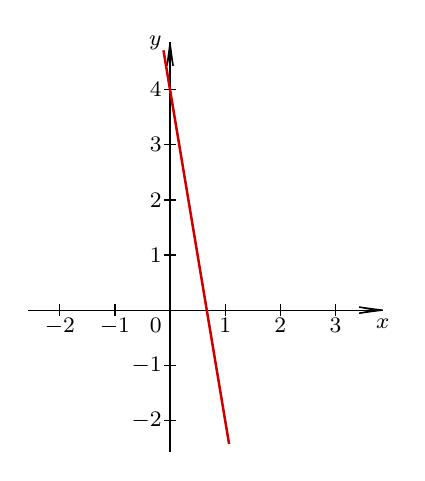
\begin{tikzpicture}
                            % \clip (0,0) rectangle (14.000000,10.000000);
                            {\footnotesize
                            
                            % Drawing 2D Cartesian system
                            \draw (3.000000,3.000000) node [anchor=north east] { $0$ };%
                            \draw [line width=0.016cm] (3.000000,2.925000) -- (3.000000,3.075000);%
                            \draw (3.700000,3.000000) node [anchor=north] { $1$ };%
                            \draw [line width=0.016cm] (3.700000,2.925000) -- (3.700000,3.075000);%
                            \draw (4.400000,3.000000) node [anchor=north] { $2$ };%
                            \draw [line width=0.016cm] (4.400000,2.925000) -- (4.400000,3.075000);%
                            \draw (5.100000,3.000000) node [anchor=north] { $3$ };%
                            \draw [line width=0.016cm] (5.100000,2.925000) -- (5.100000,3.075000);%
                            \draw (2.300000,3.000000) node [anchor=north] { $-1$ };%
                            \draw [line width=0.016cm] (2.300000,2.925000) -- (2.300000,3.075000);%
                            \draw (1.600000,3.000000) node [anchor=north] { $-2$ };%
                            \draw [line width=0.016cm] (1.600000,2.925000) -- (1.600000,3.075000);%
                            \draw (3.000000,3.700000) node [anchor=east] { $1$ };%
                            \draw [line width=0.016cm] (2.925000,3.700000) -- (3.075000,3.700000);%
                            \draw (3.000000,4.400000) node [anchor=east] { $2$ };%
                            \draw [line width=0.016cm] (2.925000,4.400000) -- (3.075000,4.400000);%
                            \draw (3.000000,5.100000) node [anchor=east] { $3$ };%
                            \draw [line width=0.016cm] (2.925000,5.100000) -- (3.075000,5.100000);%
                            \draw (3.000000,5.800000) node [anchor=east] { $4$ };%
                            \draw [line width=0.016cm] (2.925000,5.800000) -- (3.075000,5.800000);%
                            \draw (3.000000,2.300000) node [anchor=east] { $-1$ };%
                            \draw [line width=0.016cm] (2.925000,2.300000) -- (3.075000,2.300000);%
                            \draw (3.000000,1.600000) node [anchor=east] { $-2$ };%
                            \draw [line width=0.016cm] (2.925000,1.600000) -- (3.075000,1.600000);%
                            \draw (5.700000,3.000000) node [anchor=north] { $x$ };%
                            \draw (3.000000,6.400000) node [anchor=east] { $y$ };%
                            \draw [line width=0.016cm] (1.200000,3.000000) -- (5.700000,3.000000);%
                            \draw [line width=0.016cm] (5.402567,3.039158) -- (5.700000,3.000000);%
                            \draw [line width=0.016cm] (5.402567,3.039158) -- (5.600000,3.000000);%
                            \draw [line width=0.016cm] (5.402567,2.960842) -- (5.700000,3.000000);%
                            \draw [line width=0.016cm] (5.402567,2.960842) -- (5.600000,3.000000);%
                            \draw [line width=0.016cm] (3.000000,1.200000) -- (3.000000,6.400000);%
                            \draw [line width=0.016cm] (2.960842,6.102567) -- (3.000000,6.400000);%
                            \draw [line width=0.016cm] (2.960842,6.102567) -- (3.000000,6.300000);%
                            \draw [line width=0.016cm] (3.039158,6.102567) -- (3.000000,6.400000);%
                            \draw [line width=0.016cm] (3.039158,6.102567) -- (3.000000,6.300000);%
                            
                            % Changing color 204 0 0
                            \definecolor{r204g0b0}{rgb}{0.800000,0.000000,0.000000}%
                            \color{r204g0b0}% 
                            
                            % Drawing line l
                            \draw [line width=0.032cm] (3.750000,1.300000) -- (2.916667,6.300000);%
                            \color{black}
                            }
                            \end{tikzpicture}
                            
                    \end{figure}

                    \column{0.32\textwidth}
                    \vskip-1.5em
                    \begin{figure}[H]
                        \begin{tikzpicture}
                            % \clip (0,0) rectangle (14.000000,10.000000);
                            {\footnotesize
                            
                            % Drawing 2D Cartesian system
                            \draw (3.000000,3.000000) node [anchor=north east] { $0$ };%
                            \draw [line width=0.016cm] (3.000000,2.925000) -- (3.000000,3.075000);%
                            \draw (3.700000,3.000000) node [anchor=north] { $1$ };%
                            \draw [line width=0.016cm] (3.700000,2.925000) -- (3.700000,3.075000);%
                            \draw (4.400000,3.000000) node [anchor=north] { $2$ };%
                            \draw [line width=0.016cm] (4.400000,2.925000) -- (4.400000,3.075000);%
                            \draw (5.100000,3.000000) node [anchor=north] { $3$ };%
                            \draw [line width=0.016cm] (5.100000,2.925000) -- (5.100000,3.075000);%
                            \draw (2.300000,3.000000) node [anchor=north] { $-1$ };%
                            \draw [line width=0.016cm] (2.300000,2.925000) -- (2.300000,3.075000);%
                            \draw (1.600000,3.000000) node [anchor=north] { $-2$ };%
                            \draw [line width=0.016cm] (1.600000,2.925000) -- (1.600000,3.075000);%
                            \draw (3.000000,3.700000) node [anchor=east] { $1$ };%
                            \draw [line width=0.016cm] (2.925000,3.700000) -- (3.075000,3.700000);%
                            \draw (3.000000,4.400000) node [anchor=east] { $2$ };%
                            \draw [line width=0.016cm] (2.925000,4.400000) -- (3.075000,4.400000);%
                            \draw (3.000000,5.100000) node [anchor=east] { $3$ };%
                            \draw [line width=0.016cm] (2.925000,5.100000) -- (3.075000,5.100000);%
                            \draw (3.000000,5.800000) node [anchor=east] { $4$ };%
                            \draw [line width=0.016cm] (2.925000,5.800000) -- (3.075000,5.800000);%
                            \draw (3.000000,2.300000) node [anchor=east] { $-1$ };%
                            \draw [line width=0.016cm] (2.925000,2.300000) -- (3.075000,2.300000);%
                            \draw (3.000000,1.600000) node [anchor=east] { $-2$ };%
                            \draw [line width=0.016cm] (2.925000,1.600000) -- (3.075000,1.600000);%
                            \draw (5.700000,3.000000) node [anchor=north] { $x$ };%
                            \draw (3.000000,6.400000) node [anchor=east] { $y$ };%
                            \draw [line width=0.016cm] (1.200000,3.000000) -- (5.700000,3.000000);%
                            \draw [line width=0.016cm] (5.402567,3.039158) -- (5.700000,3.000000);%
                            \draw [line width=0.016cm] (5.402567,3.039158) -- (5.600000,3.000000);%
                            \draw [line width=0.016cm] (5.402567,2.960842) -- (5.700000,3.000000);%
                            \draw [line width=0.016cm] (5.402567,2.960842) -- (5.600000,3.000000);%
                            \draw [line width=0.016cm] (3.000000,1.200000) -- (3.000000,6.400000);%
                            \draw [line width=0.016cm] (2.960842,6.102567) -- (3.000000,6.400000);%
                            \draw [line width=0.016cm] (2.960842,6.102567) -- (3.000000,6.300000);%
                            \draw [line width=0.016cm] (3.039158,6.102567) -- (3.000000,6.400000);%
                            \draw [line width=0.016cm] (3.039158,6.102567) -- (3.000000,6.300000);%
                            
                            % Changing color 204 0 0
                            \definecolor{r204g0b0}{rgb}{0.800000,0.000000,0.000000}%
                            \color{r204g0b0}% 
                            
                            % Drawing line l
                            \draw [line width=0.032cm] (4.900000,6.300000) -- (1.300000,2.700000);%
                            \color{black}
                            }
                            \end{tikzpicture}
                            
                    \end{figure}

                \end{columns}

            \end{exampleblock}}

        \end{frame}


        \begin{frame}
            \only<2->{\begin{exampleblock}{Naloga}
                Zapišite predpis linearne funkcije, ki jo prikzauje graf.

                \begin{columns}
                    \column{0.32\textwidth}
                    \vskip-1.5em
                    \begin{figure}[H]
                        \begin{tikzpicture}
                            % \clip (0,0) rectangle (14.000000,10.000000);
                            {\footnotesize
                            
                            % Drawing 2D Cartesian system
                            \draw (3.000000,3.000000) node [anchor=north east] { $0$ };%
                            \draw [line width=0.016cm] (3.000000,2.925000) -- (3.000000,3.075000);%
                            \draw (3.700000,3.000000) node [anchor=north] { $1$ };%
                            \draw [line width=0.016cm] (3.700000,2.925000) -- (3.700000,3.075000);%
                            \draw (4.400000,3.000000) node [anchor=north] { $2$ };%
                            \draw [line width=0.016cm] (4.400000,2.925000) -- (4.400000,3.075000);%
                            \draw (5.100000,3.000000) node [anchor=north] { $3$ };%
                            \draw [line width=0.016cm] (5.100000,2.925000) -- (5.100000,3.075000);%
                            \draw (2.300000,3.000000) node [anchor=north] { $-1$ };%
                            \draw [line width=0.016cm] (2.300000,2.925000) -- (2.300000,3.075000);%
                            \draw (1.600000,3.000000) node [anchor=north] { $-2$ };%
                            \draw [line width=0.016cm] (1.600000,2.925000) -- (1.600000,3.075000);%
                            \draw (3.000000,3.700000) node [anchor=east] { $1$ };%
                            \draw [line width=0.016cm] (2.925000,3.700000) -- (3.075000,3.700000);%
                            \draw (3.000000,4.400000) node [anchor=east] { $2$ };%
                            \draw [line width=0.016cm] (2.925000,4.400000) -- (3.075000,4.400000);%
                            \draw (3.000000,5.100000) node [anchor=east] { $3$ };%
                            \draw [line width=0.016cm] (2.925000,5.100000) -- (3.075000,5.100000);%
                            \draw (3.000000,5.800000) node [anchor=east] { $4$ };%
                            \draw [line width=0.016cm] (2.925000,5.800000) -- (3.075000,5.800000);%
                            \draw (3.000000,2.300000) node [anchor=east] { $-1$ };%
                            \draw [line width=0.016cm] (2.925000,2.300000) -- (3.075000,2.300000);%
                            \draw (3.000000,1.600000) node [anchor=east] { $-2$ };%
                            \draw [line width=0.016cm] (2.925000,1.600000) -- (3.075000,1.600000);%
                            \draw (5.700000,3.000000) node [anchor=north] { $x$ };%
                            \draw (3.000000,6.400000) node [anchor=east] { $y$ };%
                            \draw [line width=0.016cm] (1.200000,3.000000) -- (5.700000,3.000000);%
                            \draw [line width=0.016cm] (5.402567,3.039158) -- (5.700000,3.000000);%
                            \draw [line width=0.016cm] (5.402567,3.039158) -- (5.600000,3.000000);%
                            \draw [line width=0.016cm] (5.402567,2.960842) -- (5.700000,3.000000);%
                            \draw [line width=0.016cm] (5.402567,2.960842) -- (5.600000,3.000000);%
                            \draw [line width=0.016cm] (3.000000,1.200000) -- (3.000000,6.400000);%
                            \draw [line width=0.016cm] (2.960842,6.102567) -- (3.000000,6.400000);%
                            \draw [line width=0.016cm] (2.960842,6.102567) -- (3.000000,6.300000);%
                            \draw [line width=0.016cm] (3.039158,6.102567) -- (3.000000,6.400000);%
                            \draw [line width=0.016cm] (3.039158,6.102567) -- (3.000000,6.300000);%
                            
                            % Changing color 204 0 0
                            \definecolor{r204g0b0}{rgb}{0.800000,0.000000,0.000000}%
                            \color{r204g0b0}% 
                            
                            % Drawing line l
                            \draw [line width=0.032cm] (1.300000,3.700000) -- (5.600000,3.700000);%
                            \color{black}
                            }
                            \end{tikzpicture}
                                                             
                    \end{figure}

                    \column{0.32\textwidth}
                    \vskip-1.5em
                    \begin{figure}[H]
                        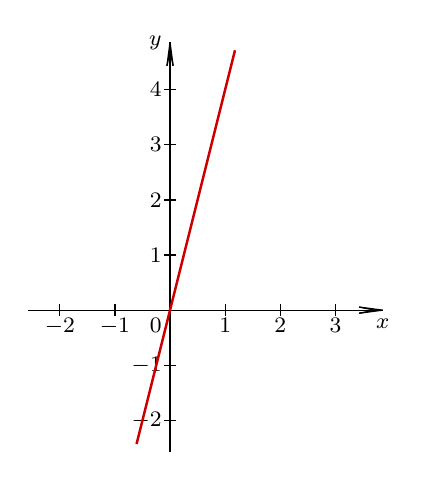
\begin{tikzpicture}
                            % \clip (0,0) rectangle (14.000000,10.000000);
                            {\footnotesize
                            
                            % Drawing 2D Cartesian system
                            \draw (3.000000,3.000000) node [anchor=north east] { $0$ };%
                            \draw [line width=0.016cm] (3.000000,2.925000) -- (3.000000,3.075000);%
                            \draw (3.700000,3.000000) node [anchor=north] { $1$ };%
                            \draw [line width=0.016cm] (3.700000,2.925000) -- (3.700000,3.075000);%
                            \draw (4.400000,3.000000) node [anchor=north] { $2$ };%
                            \draw [line width=0.016cm] (4.400000,2.925000) -- (4.400000,3.075000);%
                            \draw (5.100000,3.000000) node [anchor=north] { $3$ };%
                            \draw [line width=0.016cm] (5.100000,2.925000) -- (5.100000,3.075000);%
                            \draw (2.300000,3.000000) node [anchor=north] { $-1$ };%
                            \draw [line width=0.016cm] (2.300000,2.925000) -- (2.300000,3.075000);%
                            \draw (1.600000,3.000000) node [anchor=north] { $-2$ };%
                            \draw [line width=0.016cm] (1.600000,2.925000) -- (1.600000,3.075000);%
                            \draw (3.000000,3.700000) node [anchor=east] { $1$ };%
                            \draw [line width=0.016cm] (2.925000,3.700000) -- (3.075000,3.700000);%
                            \draw (3.000000,4.400000) node [anchor=east] { $2$ };%
                            \draw [line width=0.016cm] (2.925000,4.400000) -- (3.075000,4.400000);%
                            \draw (3.000000,5.100000) node [anchor=east] { $3$ };%
                            \draw [line width=0.016cm] (2.925000,5.100000) -- (3.075000,5.100000);%
                            \draw (3.000000,5.800000) node [anchor=east] { $4$ };%
                            \draw [line width=0.016cm] (2.925000,5.800000) -- (3.075000,5.800000);%
                            \draw (3.000000,2.300000) node [anchor=east] { $-1$ };%
                            \draw [line width=0.016cm] (2.925000,2.300000) -- (3.075000,2.300000);%
                            \draw (3.000000,1.600000) node [anchor=east] { $-2$ };%
                            \draw [line width=0.016cm] (2.925000,1.600000) -- (3.075000,1.600000);%
                            \draw (5.700000,3.000000) node [anchor=north] { $x$ };%
                            \draw (3.000000,6.400000) node [anchor=east] { $y$ };%
                            \draw [line width=0.016cm] (1.200000,3.000000) -- (5.700000,3.000000);%
                            \draw [line width=0.016cm] (5.402567,3.039158) -- (5.700000,3.000000);%
                            \draw [line width=0.016cm] (5.402567,3.039158) -- (5.600000,3.000000);%
                            \draw [line width=0.016cm] (5.402567,2.960842) -- (5.700000,3.000000);%
                            \draw [line width=0.016cm] (5.402567,2.960842) -- (5.600000,3.000000);%
                            \draw [line width=0.016cm] (3.000000,1.200000) -- (3.000000,6.400000);%
                            \draw [line width=0.016cm] (2.960842,6.102567) -- (3.000000,6.400000);%
                            \draw [line width=0.016cm] (2.960842,6.102567) -- (3.000000,6.300000);%
                            \draw [line width=0.016cm] (3.039158,6.102567) -- (3.000000,6.400000);%
                            \draw [line width=0.016cm] (3.039158,6.102567) -- (3.000000,6.300000);%
                            
                            % Changing color 204 0 0
                            \definecolor{r204g0b0}{rgb}{0.800000,0.000000,0.000000}%
                            \color{r204g0b0}% 
                            
                            % Drawing line l
                            \draw [line width=0.032cm] (2.575000,1.300000) -- (3.825000,6.300000);%
                            \color{black}
                            }
                            \end{tikzpicture}
                            
                    \end{figure}

                    \column{0.32\textwidth}
                    \vskip-1.5em
                    \begin{figure}[H]
                        \begin{tikzpicture}
                            % \clip (0,0) rectangle (14.000000,10.000000);
                            {\footnotesize
                            
                            % Drawing 2D Cartesian system
                            \draw (3.000000,3.000000) node [anchor=north east] { $0$ };%
                            \draw [line width=0.016cm] (3.000000,2.925000) -- (3.000000,3.075000);%
                            \draw (3.700000,3.000000) node [anchor=north] { $1$ };%
                            \draw [line width=0.016cm] (3.700000,2.925000) -- (3.700000,3.075000);%
                            \draw (4.400000,3.000000) node [anchor=north] { $2$ };%
                            \draw [line width=0.016cm] (4.400000,2.925000) -- (4.400000,3.075000);%
                            \draw (5.100000,3.000000) node [anchor=north] { $3$ };%
                            \draw [line width=0.016cm] (5.100000,2.925000) -- (5.100000,3.075000);%
                            \draw (2.300000,3.000000) node [anchor=north] { $-1$ };%
                            \draw [line width=0.016cm] (2.300000,2.925000) -- (2.300000,3.075000);%
                            \draw (1.600000,3.000000) node [anchor=north] { $-2$ };%
                            \draw [line width=0.016cm] (1.600000,2.925000) -- (1.600000,3.075000);%
                            \draw (3.000000,3.700000) node [anchor=east] { $1$ };%
                            \draw [line width=0.016cm] (2.925000,3.700000) -- (3.075000,3.700000);%
                            \draw (3.000000,4.400000) node [anchor=east] { $2$ };%
                            \draw [line width=0.016cm] (2.925000,4.400000) -- (3.075000,4.400000);%
                            \draw (3.000000,5.100000) node [anchor=east] { $3$ };%
                            \draw [line width=0.016cm] (2.925000,5.100000) -- (3.075000,5.100000);%
                            \draw (3.000000,5.800000) node [anchor=east] { $4$ };%
                            \draw [line width=0.016cm] (2.925000,5.800000) -- (3.075000,5.800000);%
                            \draw (3.000000,2.300000) node [anchor=east] { $-1$ };%
                            \draw [line width=0.016cm] (2.925000,2.300000) -- (3.075000,2.300000);%
                            \draw (3.000000,1.600000) node [anchor=east] { $-2$ };%
                            \draw [line width=0.016cm] (2.925000,1.600000) -- (3.075000,1.600000);%
                            \draw (5.700000,3.000000) node [anchor=north] { $x$ };%
                            \draw (3.000000,6.400000) node [anchor=east] { $y$ };%
                            \draw [line width=0.016cm] (1.200000,3.000000) -- (5.700000,3.000000);%
                            \draw [line width=0.016cm] (5.402567,3.039158) -- (5.700000,3.000000);%
                            \draw [line width=0.016cm] (5.402567,3.039158) -- (5.600000,3.000000);%
                            \draw [line width=0.016cm] (5.402567,2.960842) -- (5.700000,3.000000);%
                            \draw [line width=0.016cm] (5.402567,2.960842) -- (5.600000,3.000000);%
                            \draw [line width=0.016cm] (3.000000,1.200000) -- (3.000000,6.400000);%
                            \draw [line width=0.016cm] (2.960842,6.102567) -- (3.000000,6.400000);%
                            \draw [line width=0.016cm] (2.960842,6.102567) -- (3.000000,6.300000);%
                            \draw [line width=0.016cm] (3.039158,6.102567) -- (3.000000,6.400000);%
                            \draw [line width=0.016cm] (3.039158,6.102567) -- (3.000000,6.300000);%
                            
                            % Changing color 204 0 0
                            \definecolor{r204g0b0}{rgb}{0.800000,0.000000,0.000000}%
                            \color{r204g0b0}% 
                            
                            % Drawing line l
                            \draw [line width=0.032cm] (2.700000,1.300000) -- (5.600000,4.200000);%
                            \color{black}
                            }
                            \end{tikzpicture}
                            
                    \end{figure}

                \end{columns}

            \end{exampleblock}}

        \end{frame}


        \begin{frame}
            \only<2->{\begin{exampleblock}{Naloga}
                Zapišite predpis linearne funkcije, ki jo prikzauje graf.

                \begin{columns}
                    \column{0.32\textwidth}
                    \vskip-1.5em
                    \begin{figure}[H]
                        \begin{tikzpicture}
                            % \clip (0,0) rectangle (14.000000,10.000000);
                            {\footnotesize
                            
                            % Drawing 2D Cartesian system
                            \draw (3.000000,3.000000) node [anchor=north east] { $0$ };%
                            \draw [line width=0.016cm] (3.000000,2.925000) -- (3.000000,3.075000);%
                            \draw (3.700000,3.000000) node [anchor=north] { $1$ };%
                            \draw [line width=0.016cm] (3.700000,2.925000) -- (3.700000,3.075000);%
                            \draw (4.400000,3.000000) node [anchor=north] { $2$ };%
                            \draw [line width=0.016cm] (4.400000,2.925000) -- (4.400000,3.075000);%
                            \draw (5.100000,3.000000) node [anchor=north] { $3$ };%
                            \draw [line width=0.016cm] (5.100000,2.925000) -- (5.100000,3.075000);%
                            \draw (2.300000,3.000000) node [anchor=north] { $-1$ };%
                            \draw [line width=0.016cm] (2.300000,2.925000) -- (2.300000,3.075000);%
                            \draw (1.600000,3.000000) node [anchor=north] { $-2$ };%
                            \draw [line width=0.016cm] (1.600000,2.925000) -- (1.600000,3.075000);%
                            \draw (3.000000,3.700000) node [anchor=east] { $1$ };%
                            \draw [line width=0.016cm] (2.925000,3.700000) -- (3.075000,3.700000);%
                            \draw (3.000000,4.400000) node [anchor=east] { $2$ };%
                            \draw [line width=0.016cm] (2.925000,4.400000) -- (3.075000,4.400000);%
                            \draw (3.000000,5.100000) node [anchor=east] { $3$ };%
                            \draw [line width=0.016cm] (2.925000,5.100000) -- (3.075000,5.100000);%
                            \draw (3.000000,5.800000) node [anchor=east] { $4$ };%
                            \draw [line width=0.016cm] (2.925000,5.800000) -- (3.075000,5.800000);%
                            \draw (3.000000,2.300000) node [anchor=east] { $-1$ };%
                            \draw [line width=0.016cm] (2.925000,2.300000) -- (3.075000,2.300000);%
                            \draw (3.000000,1.600000) node [anchor=east] { $-2$ };%
                            \draw [line width=0.016cm] (2.925000,1.600000) -- (3.075000,1.600000);%
                            \draw (5.700000,3.000000) node [anchor=north] { $x$ };%
                            \draw (3.000000,6.400000) node [anchor=east] { $y$ };%
                            \draw [line width=0.016cm] (1.200000,3.000000) -- (5.700000,3.000000);%
                            \draw [line width=0.016cm] (5.402567,3.039158) -- (5.700000,3.000000);%
                            \draw [line width=0.016cm] (5.402567,3.039158) -- (5.600000,3.000000);%
                            \draw [line width=0.016cm] (5.402567,2.960842) -- (5.700000,3.000000);%
                            \draw [line width=0.016cm] (5.402567,2.960842) -- (5.600000,3.000000);%
                            \draw [line width=0.016cm] (3.000000,1.200000) -- (3.000000,6.400000);%
                            \draw [line width=0.016cm] (2.960842,6.102567) -- (3.000000,6.400000);%
                            \draw [line width=0.016cm] (2.960842,6.102567) -- (3.000000,6.300000);%
                            \draw [line width=0.016cm] (3.039158,6.102567) -- (3.000000,6.400000);%
                            \draw [line width=0.016cm] (3.039158,6.102567) -- (3.000000,6.300000);%
                            
                            % Changing color 204 0 0
                            \definecolor{r204g0b0}{rgb}{0.800000,0.000000,0.000000}%
                            \color{r204g0b0}% 
                            
                            % Drawing line l
                            \draw [line width=0.032cm] (1.300000,3.550000) -- (5.600000,5.700000);%
                            \color{black}
                            }
                            \end{tikzpicture}
                                                  
                    \end{figure}

                    \column{0.32\textwidth}
                    \vskip-1.5em
                    \begin{figure}[H]
                        \begin{tikzpicture}
                            % \clip (0,0) rectangle (14.000000,10.000000);
                            {\footnotesize
                            
                            % Drawing 2D Cartesian system
                            \draw (3.000000,3.000000) node [anchor=north east] { $0$ };%
                            \draw [line width=0.016cm] (3.000000,2.925000) -- (3.000000,3.075000);%
                            \draw (3.700000,3.000000) node [anchor=north] { $1$ };%
                            \draw [line width=0.016cm] (3.700000,2.925000) -- (3.700000,3.075000);%
                            \draw (4.400000,3.000000) node [anchor=north] { $2$ };%
                            \draw [line width=0.016cm] (4.400000,2.925000) -- (4.400000,3.075000);%
                            \draw (5.100000,3.000000) node [anchor=north] { $3$ };%
                            \draw [line width=0.016cm] (5.100000,2.925000) -- (5.100000,3.075000);%
                            \draw (2.300000,3.000000) node [anchor=north] { $-1$ };%
                            \draw [line width=0.016cm] (2.300000,2.925000) -- (2.300000,3.075000);%
                            \draw (1.600000,3.000000) node [anchor=north] { $-2$ };%
                            \draw [line width=0.016cm] (1.600000,2.925000) -- (1.600000,3.075000);%
                            \draw (3.000000,3.700000) node [anchor=east] { $1$ };%
                            \draw [line width=0.016cm] (2.925000,3.700000) -- (3.075000,3.700000);%
                            \draw (3.000000,4.400000) node [anchor=east] { $2$ };%
                            \draw [line width=0.016cm] (2.925000,4.400000) -- (3.075000,4.400000);%
                            \draw (3.000000,5.100000) node [anchor=east] { $3$ };%
                            \draw [line width=0.016cm] (2.925000,5.100000) -- (3.075000,5.100000);%
                            \draw (3.000000,5.800000) node [anchor=east] { $4$ };%
                            \draw [line width=0.016cm] (2.925000,5.800000) -- (3.075000,5.800000);%
                            \draw (3.000000,2.300000) node [anchor=east] { $-1$ };%
                            \draw [line width=0.016cm] (2.925000,2.300000) -- (3.075000,2.300000);%
                            \draw (3.000000,1.600000) node [anchor=east] { $-2$ };%
                            \draw [line width=0.016cm] (2.925000,1.600000) -- (3.075000,1.600000);%
                            \draw (5.700000,3.000000) node [anchor=north] { $x$ };%
                            \draw (3.000000,6.400000) node [anchor=east] { $y$ };%
                            \draw [line width=0.016cm] (1.200000,3.000000) -- (5.700000,3.000000);%
                            \draw [line width=0.016cm] (5.402567,3.039158) -- (5.700000,3.000000);%
                            \draw [line width=0.016cm] (5.402567,3.039158) -- (5.600000,3.000000);%
                            \draw [line width=0.016cm] (5.402567,2.960842) -- (5.700000,3.000000);%
                            \draw [line width=0.016cm] (5.402567,2.960842) -- (5.600000,3.000000);%
                            \draw [line width=0.016cm] (3.000000,1.200000) -- (3.000000,6.400000);%
                            \draw [line width=0.016cm] (2.960842,6.102567) -- (3.000000,6.400000);%
                            \draw [line width=0.016cm] (2.960842,6.102567) -- (3.000000,6.300000);%
                            \draw [line width=0.016cm] (3.039158,6.102567) -- (3.000000,6.400000);%
                            \draw [line width=0.016cm] (3.039158,6.102567) -- (3.000000,6.300000);%
                            
                            % Changing color 204 0 0
                            \definecolor{r204g0b0}{rgb}{0.800000,0.000000,0.000000}%
                            \color{r204g0b0}% 
                            
                            % Drawing line l
                            \draw [line width=0.032cm] (4.700000,1.300000) -- (1.300000,4.700000);%
                            \color{black}
                            }
                            \end{tikzpicture}
                            
                    \end{figure}

                    \column{0.32\textwidth}
                    \vskip-1.5em
                    \begin{figure}[H]
                        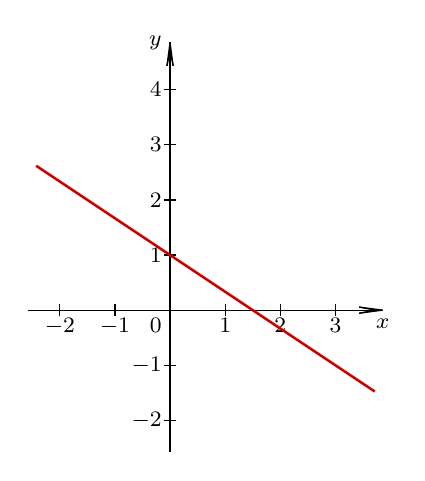
\begin{tikzpicture}
                            % \clip (0,0) rectangle (14.000000,10.000000);
                            {\footnotesize
                            
                            % Drawing 2D Cartesian system
                            \draw (3.000000,3.000000) node [anchor=north east] { $0$ };%
                            \draw [line width=0.016cm] (3.000000,2.925000) -- (3.000000,3.075000);%
                            \draw (3.700000,3.000000) node [anchor=north] { $1$ };%
                            \draw [line width=0.016cm] (3.700000,2.925000) -- (3.700000,3.075000);%
                            \draw (4.400000,3.000000) node [anchor=north] { $2$ };%
                            \draw [line width=0.016cm] (4.400000,2.925000) -- (4.400000,3.075000);%
                            \draw (5.100000,3.000000) node [anchor=north] { $3$ };%
                            \draw [line width=0.016cm] (5.100000,2.925000) -- (5.100000,3.075000);%
                            \draw (2.300000,3.000000) node [anchor=north] { $-1$ };%
                            \draw [line width=0.016cm] (2.300000,2.925000) -- (2.300000,3.075000);%
                            \draw (1.600000,3.000000) node [anchor=north] { $-2$ };%
                            \draw [line width=0.016cm] (1.600000,2.925000) -- (1.600000,3.075000);%
                            \draw (3.000000,3.700000) node [anchor=east] { $1$ };%
                            \draw [line width=0.016cm] (2.925000,3.700000) -- (3.075000,3.700000);%
                            \draw (3.000000,4.400000) node [anchor=east] { $2$ };%
                            \draw [line width=0.016cm] (2.925000,4.400000) -- (3.075000,4.400000);%
                            \draw (3.000000,5.100000) node [anchor=east] { $3$ };%
                            \draw [line width=0.016cm] (2.925000,5.100000) -- (3.075000,5.100000);%
                            \draw (3.000000,5.800000) node [anchor=east] { $4$ };%
                            \draw [line width=0.016cm] (2.925000,5.800000) -- (3.075000,5.800000);%
                            \draw (3.000000,2.300000) node [anchor=east] { $-1$ };%
                            \draw [line width=0.016cm] (2.925000,2.300000) -- (3.075000,2.300000);%
                            \draw (3.000000,1.600000) node [anchor=east] { $-2$ };%
                            \draw [line width=0.016cm] (2.925000,1.600000) -- (3.075000,1.600000);%
                            \draw (5.700000,3.000000) node [anchor=north] { $x$ };%
                            \draw (3.000000,6.400000) node [anchor=east] { $y$ };%
                            \draw [line width=0.016cm] (1.200000,3.000000) -- (5.700000,3.000000);%
                            \draw [line width=0.016cm] (5.402567,3.039158) -- (5.700000,3.000000);%
                            \draw [line width=0.016cm] (5.402567,3.039158) -- (5.600000,3.000000);%
                            \draw [line width=0.016cm] (5.402567,2.960842) -- (5.700000,3.000000);%
                            \draw [line width=0.016cm] (5.402567,2.960842) -- (5.600000,3.000000);%
                            \draw [line width=0.016cm] (3.000000,1.200000) -- (3.000000,6.400000);%
                            \draw [line width=0.016cm] (2.960842,6.102567) -- (3.000000,6.400000);%
                            \draw [line width=0.016cm] (2.960842,6.102567) -- (3.000000,6.300000);%
                            \draw [line width=0.016cm] (3.039158,6.102567) -- (3.000000,6.400000);%
                            \draw [line width=0.016cm] (3.039158,6.102567) -- (3.000000,6.300000);%
                            
                            % Changing color 204 0 0
                            \definecolor{r204g0b0}{rgb}{0.800000,0.000000,0.000000}%
                            \color{r204g0b0}% 
                            
                            % Drawing line l
                            \draw [line width=0.032cm] (1.300000,4.833220) -- (5.600000,1.966840);%
                            \color{black}
                            }
                            \end{tikzpicture}
                            
                    \end{figure}

                \end{columns}

            \end{exampleblock}}

        \end{frame}


        \begin{frame}
            \only<2->{\begin{exampleblock}{Naloga}
                Narišite graf sestavljene funkcije in zapišite njeno zalogo vrednosti.
                \vskip-1em
                \begin{columns}
                    \column{0.5\textwidth}
                    \begin{itemize}
                        \item $f(x)=\begin{cases}
                            2x; & x\leq 2 \\ 4; &x>2
                        \end{cases}$ \\~\\~
                        \item $g(x)=\begin{cases}
                            x+3; & x\leq -2 \\ -x-1; &x>-2
                        \end{cases}$ \\~\\~
                        \item $h(x)=\begin{cases}
                            x; & x\leq 1 \\ -1; & x>1
                        \end{cases}$ \\~\\~
                    \end{itemize}

                    \column{0.47\textwidth}
                    \begin{itemize}
                        \item $k(x)=\begin{cases}
                            -x+1; & x\leq 2 \\ -1; &2<x<4 \\ x-5; &x\geq 4
                        \end{cases}$ \\~\\~
                        \item $l(x)=\begin{cases}
                            0.5x; & x\leq 2 \\ 2x-3; &2<x<4 \\ 0.5x+3; &x\geq 4
                        \end{cases}$ \\~\\~
                    \end{itemize}
                \end{columns}

            \end{exampleblock}}
        \end{frame}


        \begin{frame}
            \only<2->{\begin{exampleblock}{Naloga}
                Narišite graf funkcije. 
                \vskip-1em
                \begin{columns}
                    \column{0.5\textwidth}
                    \begin{itemize}
                        \item $f(x)=|3x-3|$ \\~
                        \item $g(x)=|2x+1|+1$ \\~
                        \item $h(x)=1-|x+1|$ \\~
                        \item $i(x)=3-|2x-1|$ \\~
                    \end{itemize}

                    \column{0.47\textwidth}
                    \begin{itemize}
                        \item $j(x)=x+|x-2|$ \\~
                        \item $k(x)=|x+1|-2$ \\~
                        \item $l(x)=-|0.5x+3|$ \\~
                        \item $m(x)=3-|x-2|$ \\~
                    \end{itemize}
                \end{columns}

            \end{exampleblock}}
        \end{frame}
